\documentclass{book}

\usepackage[left=2.5cm, right=2.5cm, top=2cm, bottom=2cm]{geometry}

\usepackage{tikz-cd}
% % math mode additions
\usepackage{amsmath}
\usepackage{amsfonts}
\usepackage{amssymb}

% nice differentation
% ISO: Get straight d's when differantiating
\usepackage[ISO]{diffcoeff}

% \usepackage{physics}

\usepackage{slashed}

% nice 3-vectors
\usepackage{esvect}

% appendix
\usepackage[title]{appendix}
\usepackage{pdfpages}
 
\usepackage[export]{adjustbox}

% in-document references
\usepackage{hyperref}

% Nice table of contents
\usepackage{tocloft}

% Get floats right
\usepackage[section]{placeins}

% adjust fig captions
\usepackage{caption}
\usepackage{subcaption}
\captionsetup{width=.9\textwidth}

% \usepackage{titlepic}
\usepackage[prependcaption,textsize=tiny]{todonotes}
\usepackage{xpatch}

\usepackage{setspace}


\usepackage[%
    style=numeric-comp,
    sorting=none,
    sortcites=true,
    doi=true,
    url=false,
    giveninits=true,
    hyperref
    ]{biblatex}

\setlength{\marginparwidth}{2.2cm}
% \setlength\cftparskip{1pt}
% \setlength\cftbeforechapskip{0pt}

% space instead of indentation for paragraphs

% \def\equationautorefname~#1\null{Eq.~(#1)\null}


% Chiral pertubation theory
\newcommand{\chpt}[0]{\ensuremath{\chi \text{PT}}} 
% Lagrangian L
\newcommand{\Ell}{\mathcal{L}}
% Hamiltonian H
\newcommand{\He}{\mathcal{H}}
% Potential V
\newcommand{\Ve}{\mathcal{V}}
% effective potential
\newcommand{\Veff}{\mathcal{V}_{\mathrm{eff}}}
% Manifold M
\newcommand{\Em}{\mathcal{M}}
% Fancy f
\newcommand{\Eff}{\mathcal{F}}
\newcommand{\Oh}{\mathcal O}
% Real numbers
\newcommand{\R}{\mathbb{R}}
% Funcitonal integral D
\newcommand{\D}{\mathcal D}
\newcommand{\id}{\mathrm{id}}
\newcommand{\const}{\mathrm{const.}}
% Identity matice/operation
\newcommand{\one}{\text{\usefont{U}{bbold}{m}{n}1}}
\MakeRobust{\one}
%! Fix these
\newcommand{\Olie}{\text O}
\newcommand{\SO}{\text{SO}}

% operator in braket
\newcommand{\inner}[3]{\left\langle #1 {\left| #2 \right|} #3 \right\rangle}
% expectationvalue
\newcommand{\ex}[1]{\left\langle #1 \right\rangle}

% Set builder notation
\newcommand{\setbuilder}[2]{\left\{\, #1 \mid #2 \,\right\}}
% Time ordering operator
\newcommand{\T}[1]{\textrm{T} \left\{ #1 \right\}}

% Using diffcoeff instead
% \newcommand{\}{\fdv}
 

% Floor function
\DeclarePairedDelimiter\floor{\lfloor}{\rfloor}
\DeclareMathOperator{\arcsinh}{arcsinh}



\title{\huge{Master}}
\author{
    \large{Martin Kjøllesdal Johnsrud }\\
    \normalsize{Supervisor: Jens Oluf Andersen}
    }


\bibliography{master}
% Supress note field in bibliography
\AtEveryBibitem{\clearfield{note}}


\begin{document}
    \maketitle
    \listoftodos
    \tableofcontents

    % \chapter{Introduction}
    % \todo{Wirte introduction}    
    % Pion stars have recently been proposed~\autocite{andersenBoseEinsteinCondensationPion2018,brandtNewClassCompact2018}.

    \chapter{General relativity and the TOV-equation}
    \label{chapter: GR}

    General relativity describes how the fabric of space and time is bent by the presence of matter and energy.
It was first written down by Einstein more than a hundred years ago, and is to this day the most accurate model we have for gravitational effects.
The theory has made numerous accurate and counterintuitive predictions, which have been borne out by experiments.
In this chapter, we will survey the basics of general relativity as well as some mathematical prerequisites.
We will then use this to derive the Tolman-Oppenheimer-Volkoff (TOV) equation.
This is a differential equation that models massive stellar objects, such as stars. 
This chapter is based on~\autocite{carrollSpacetimeGeometryIntroduction2019,leeSmoothManifolds2012}.

\section{Differential geometry}

General relativity is formulated in the language of \emph{differential geometry}, which generalizes multivariable calculus to more general spaces than $\R^n$.
Such a space is a differentiable \emph{manifold}, $\Em$.
A manifold is a set of points that are locally homeomoriphic to $\R^n$.
That is, for all points $p \in \Em$, there is a neighbourhood $U$ around $p$ and a corresponding set of continous functions,
\begin{align}
    x^\mu: U \subseteq \Em & \longmapsto V \subseteq \R^n, \\
    p & \longmapsto x^\mu(p).
\end{align}
that has a continous inverse-functions $\varphi_x$ such that $\varphi_x(x(p)) = p$ for all $p \in U$.
$x^\mu = (x^0, ..., x^{n- 1})$ are a coordinate function of $\Em$.
In the case of a differentiable manifold, these must be diffeomorphisms, i.e. infinitly differentiable.
Differentiablility of coordinate functions is defined by considering two different coordinate functions, $x^\mu$ and $x'^\mu$, with the possibliy overlapping domains $U$ and $U'$.
We can then define a function between subsets of $\R^n$ by mapping via $\Em$, the transition map  
\begin{align}
    f_{x'\rightarrow x} = x^\mu\circ\varphi_{x'} : \R^n \mapsto \R^n.
\end{align}
%
It is defined as the function which makes the following diagram commute\footnote{To be rigorous, one has to restrict the domains and image of the coordinate function when combining them. We will leave this implicit here.}
%
\begin{equation}
    \begin{tikzcd}
        \R^n \arrow[rd, "f_{x'\rightarrow x}"'] & \Em \arrow[l, "x"'] \arrow[d, "x'"] \\
        & \R^n
        \end{tikzcd}
\end{equation}
%
The map is illustrated in \autoref{fig: transition map}.
A set of functions $\mathcal A = \{x^\mu\}$ whose domain cover $\Em$ is called an \emph{atlas} of $\Em$.
If the transition function between \emph{any} two coordinate functions in the atlas is smooth, then we call the atlas smooth.
To uniquily define a differentiable manifold,  form smooth transition functions form an \emph{atlas} $\mathcal{A}$.
We then define a differentiable, or smooth, manifold as the topological manifold $\Em$ together with the \emph{maximal} atlas $\mathcal A$.
A smooth atlas is maximal if no other coordinate function can be added to the atlas while it retains its smoothness.\footnote{The maximal condition is to ensure that two equivalent atlases correspond to the same differentiable manifold. A single manifold can be combined with different maximal atlases, also called differentiable structures. }
%
\begin{figure}
    \centering
    \includegraphics[width=0.5\textwidth]{figurer/transition_map_kladsvg.pdf}
    \caption{Kladd: The transition map between two coordinates}
    \label{fig: transition map}
\end{figure}

Consider two $m$ and $n$ dimensional smooth manifolds $\Em$ and $\mathcal N$.
Let $x$ denote the coordinates on $\Em$, while $y$ denotes the coordinates on $\mathcal N$.
We can define smooth functions between these manifolds in a similar way.
Consider the function
%
\begin{equation}
    F: \Em \longmapsto \mathcal N.
\end{equation}
%
This is said to be smooth, if for all points $p \in M$, there is a set of local coordinates $x$ around $p$ and $y$ around $F(p)$ so that the map $\tilde F = y \circ F \circ x^{-1}$ is smooth.
This map is defined by the diagram
%
\begin{equation}
    % https://tikzcd.yichuanshen.de/#N4Igdg9gJgpgziAXAbVABwnAlgFyxMJZABgBoBGAXVJADcBDAGwFcYkQAdDgW3pwAsARoIAEAJQB63EAF9S6TLnyEUZYtTpNW7LrwEBjJiICys+SAzY8BIuVLqaDFm0SceffocYiAcmYVWyrYUGk7arroewuIShDIaMFAA5vBEoABmAE4Q0oh2IDgQSGQgjPSCMIwACorWKqUw6TggjlouIAAe-iBZOUj5hUgATK3O7OndvbkjBUWIAMyj4SAAnpPZuSWDC0vtSbKUMkA
\begin{tikzcd}
    \mathcal M \arrow[d, "x"] \arrow[r, "F"] & \mathcal N \arrow[d, "y"] \\
    \mathbb R^m \arrow[r, "\tilde F"]               & \mathbb R^n              
    \end{tikzcd}
    %
\end{equation}
%
%
We will not be careful with  the distinction between $F$, the funciton between the abstract manifolds, and $\tilde F$, the function of theri coordinates, but rather denote both by $F(x)$.
We may take the partial derivative of such a function with respect to the coordinates $x$, $\diffp{F}/{x^\mu}$.
However, this is obviously dependent on our choice of coordinates, as a set of local coordinates can always be scaled.
To get a coordinate-independent quantity, we have to introduce the tangent space and the metric.

\subsection*{Vectors and tensors}

A curve $\gamma$ through $\Em$ i a function from $\R$ to $\Em$,
%
\begin{align}
    \gamma : \R &\longmapsto \Em \\
    \lambda & \longmapsto \gamma(\lambda).
\end{align}
%
Such curves are often denote only by their coordinates and the parameter $\lambda$, $x^\mu(\lambda) = (x^\mu \circ \gamma)(\lambda)$.
Such a curve defines a directional derivative of a real valued function $f: \Em \mapsto \R$.
Assume $\gamma(\lambda = 0) = p$.
As we are always taking the derivative of functions between $\R^n$, for different $n$, we can use the chaine rule.
The directional derivative of $f$ at $p$, given by this curve $\gamma$, is then
%
\begin{equation}
    \diff{}{\lambda} f(x(\lambda)) \bigg |_p = \diff{x^\mu}{\lambda} \bigg |_{\lambda = 0}  \diffp{}{x^\mu} f(x) \bigg |_p.
\end{equation}
%
The set of all such directional derivatives at $p$ form a vector space, $T_p \Em$, called the \emph{tangent space}.
The coordinates $x^\mu$ induce a basis of this vectorspace, 
%
\begin{equation}
    e_\mu = \diffp{}{x^\mu} = \partial_\mu,
\end{equation}
%
so any element $v \in T_p \Em$ can be written
%
\begin{equation}
    v = v^\mu \partial_\mu = \diff{x^\mu}{\lambda} \diffp{}{x^\mu}.
\end{equation}
%
Her, $\lambda$ is the parameter of the curve corresponding to the directional derivative $v$.\footnote{There is not only one curve corresponding to any directional derivative, but rather an equivalence class. }
It acts on funcitons $f : \Em \mapsto \R$ as
%
\begin{equation}
    v(f) = v^\mu \partial_\mu f.
\end{equation}
%

A function $F$ between two manifolds $\Em$ and $\mathcal N$ also induces a map between the tangent spaces of these manifolds.
This is the \emph{differential} of $F$ at $p$, 
%
\begin{align}
    \dd F_p: T_p \Em & \longmapsto T_p \mathcal N.
\end{align}
%
This is a directional derivative on $\mathcal N$, and is defined as
%
\begin{equation}
    \dd F_p(v) (g) = v(g \circ F),
\end{equation}
%
for functions $g : \mathcal N \mapsto \R$.
It thus acts on funcitons on $\mathcal N$ by ``extending'' the derivative $v$.
This is a linear map between vectorspaces, an may be written on component form by considering the differentials of the coordinate functions.
Denote the coordinates of $\mathcal N$ by $y^\mu$, and $y^\mu \circ F = F^\mu$.
Then,
%
\begin{equation}
    \dd F_p (\partial_\mu) (g) = \partial_\mu (g \circ F) |_p 
    = \diffp{F^\nu}{x^\mu}\bigg |_p \diffp{g}{y^\nu} \bigg  |_{F(p)}
\end{equation}
%
The differential is thus a generalization of the Jacobian of a function.
In the cas where of a real valued funciton, $f: \Em \mapsto \R$, and $g : \R \mapsto \R$, we get
%
\begin{equation}
    \dd f_p (v) (g) 
    = v(g \circ f) 
    = (v^\mu \partial_\mu f) |_p \, \diff{g}{f}\bigg  |_{f(p)},
\end{equation}
%
or more simply
%
\begin{equation}
    \dd f_p (v) = v^\mu \partial_\mu f |_p
\end{equation}
%
The differential of a real-valued function is thus a linear map from the vector-space $T_p \Em$ to the real numbers.
The set of all such maps form the \emph{dual space} of $T_p \Em$, denoted $(T_p^* \Em)$.
We can regard each of the coordinate functions as a real valued function,
%
\begin{equation}
    \dd x^\mu (\partial_\nu) = \diffp{x^\mu}{x_\nu} = \delta^\mu_\nu.
\end{equation}
%
These form a basis for $T^*_p \Em$.
We can show this by assuming $v = v^\mu \partial_\mu \in T_p \Em$.
Then, assuming $\dd f_p = \omega_\mu \dd x^\mu$, we get
%
\begin{equation}
    \dd f (v) = v^\mu \partial_\mu f = v^\mu \omega_\nu \dd x^\nu(\partial_\mu) = v^\mu \omega_\mu.
\end{equation}
%
Thus, we obtain a rigorous just justification for the classical expression 
%
\begin{equation}
    \dd f = \diffp{f}{x^\mu} \dd x^\mu,
\end{equation}
however we now interpret it as a covector-field instead of an ``infinitesimal displacement''.

This linear map from vectors to real numbers is gerneralized by \emph{tensors}.
Given a vector space $V$, general $(n, m)$ tensor $T$ is a multilinear map, which associates $n$ elements from $V$ and $m$ from its dual $V^*$ to the real numbers, i.e.
%
\begin{align}
    T: V \times V \times .... \times V^* \times .... &\longmapsto \R, \\
    (v, u...; \omega, ...) & \longmapsto T(v, u, ...; \omega, ...).
\end{align}
%
Multilinear means that $T$ is linear in each argument.
The set of all such maps is the tnesor product space $V\otimes V \otimes ... \otimes V^* \otimes ...$, a $\dim(V)^{n+m}$-dimensional vector space.
If $\{e_\mu\}$ and $\{e^\mu\}$ are the basis for $V$ and $V^*$, then we can write the basis of this of the tensor product space as $ \{e_\mu \otimes... e^\mu \otimes ... \}$.
The tensor can thus be written
%
\begin{equation}
    T = T^{\mu \nu\dots}{}_{\rho\dots} \, e_{\mu}\otimes e_\nu \otimes \dots e^\rho\otimes\dots, 
\end{equation}
%
where
%
\begin{equation}
    T^{\mu \nu\dots}{}_{\rho\dots} = T(e^\mu e^\nu, \dots; e_\rho, \dots).
\end{equation}


\subsection*{Geometries and the metric}

The metric is a symmetric, non-degenerate $(0, 2)$ tensor
%
\begin{equation}
    \dd s^2 = g_{\mu \nu} \, \dd x^\mu \otimes \dd x^\nu.
\end{equation}
%
It defines the geometry of the manifold $\Em$, and is the main object of study in general relativity.
As it is invertible, we define $g^{\mu \nu} = (g^{-1})_{\mu \nu}$, which is the components of a $(2, 0)$ tensor.
We use this to raise and lower indecies, as is done with the Minkowski metric $\eta_{\mu \nu}$ in special relativity.

Up until now, we have studied the tangent space $T_p \Em$ at one point, and the correpsonding dual and tensor product spaces.
We are, however, more interested in feilds of vectors, covectors and tensors than.
A tensor field $T$ takes the a value $T(p)$ of the tensor product space corresponding to the tangentspace at $p\in \Em$, $T_p \Em$.
We will use a vector felt to illustrate.
This vector field can be written as
%
\begin{equation}
    v(p) = v^\mu(p) \partial_\mu |_p. 
\end{equation}
%
We will mostly be working with the compontets $v^\mu$, which are functions of $\Em$.
For ease of notation, we write the vector as a funciton of the coordinates $x$, and drop leave the evaluatation at $p$ implicit.
The vector field $v(x)$ is unchanged by a coordinate-transformation $x^\mu \rightarrow \tilde x^\mu$; the coordinate has no effect on it and is only for our convinience. 
With this, we can deduce the transformation rules of the components under such a transformation:
%
\begin{equation}
    v = v^\mu \partial_\mu = v^\mu \diffp{\tilde x^\nu}{x^\mu} \tilde  \partial_\nu
    = \tilde v^\mu \tilde \partial_\mu, 
\end{equation}
%
or
%
\begin{equation}
    \tilde v^\mu = \diffp{\tilde x^\mu}{x^\nu} v^\nu.
\end{equation}
%
For covectors, it is
%
\begin{equation}
    \tilde \omega_\mu = \diffp{x^\nu}{\tilde x^\mu} \omega_\nu
\end{equation}
%
The gradient of a scalar function $f$, $\dd f = \partial_\mu f \dd x^\mu$, is a coordinate-independent derivative, as $\partial_\mu f$ follows the transformation law for covectors.
We generalize this by introducing the covariant derivative, $\nabla$, as a map from $(n, m)$ tensor fields to $(n, m+1)$ tensor fields.
When considering a scalar as a $(0, 0)$ tensor, we see that this generalizes the scalar derivative.

We assume
%
\begin{itemize}
    \item linearity: $\nabla (T + S) = \nabla T + \nabla S$.
    \item product rule: $\nabla (T \otimes S) = (\nabla T)\otimes S + T \otimes (\nabla S)$.
    \item reduces to partial derivative: $\nabla_\mu f = \partial_\mu f$.
    \item Krönecker delta gives zero: $\nabla_\mu \delta^\rho_\nu = 0$.
\end{itemize}
%
With this, we can in general write the covariant derivative as~\autocite{carrollSpacetimeGeometryIntroduction2019}
%
\begin{align}
    \nabla_\mu v^\nu &= \partial_\mu v^\mu + \Gamma^\mu_{\nu \rho} v^\rho, \\
    \nabla_\mu \omega_\nu &= \partial_\mu \omega_\nu - \Gamma^\rho_{\mu \nu} \omega^\rho,
\end{align}
%
for vectors and covectors.
$\Gamma^{\mu}_{\nu \rho}$ are called \emph{Christoffel symbols}.
The generalization for higher-order tensors is straight forward, 
%
\begin{equation}
    \nabla_\mu T^{\nu\dots}{}_{\rho\dots}
    =
    \partial_\mu T^{\nu\dots}{}_{\rho\dots}
    + \Gamma^\mu_{\nu \lambda} T^{\lambda\dots}{}_{\rho\dots} +\dots
    - \Gamma^\lambda_{\mu \rho} T^{\mu\dots}{}_{\lambda\dots} -\dots
\end{equation}
%
This is still not enough to to uniquely determin the Christoffel symbols.
We will furhtermore assume $\Gamma^{\lambda}_{\mu \nu} = \Gamma^{\lambda}_{\nu \mu}$ and $\nabla_\mu g_{\nu \rho} = 0$.
With these, we can find an explicit formula of the Christoffel symbols in terms of the metric, 
%
\begin{equation}
    \label{christoffel symbols from metric}
    \Gamma^\rho_{\mu \nu} = \frac{1}{2} g^{\rho \sigma} (\partial_\mu g_{\nu \sigma} - \partial_\sigma g_{\mu \nu} + \partial_{\nu}g_{\sigma \mu}).
\end{equation}
%

The curvature of the manifold $\Em$, with the metic $g_{\mu \nu}$, is encoded in the Riemann tensor.
It is defined by
%
\begin{equation}
    [\nabla_\mu, \nabla_\nu] v^\rho = R^{\rho}{}_{\sigma \mu \nu} v^\sigma,
\end{equation}
%
which in our case gives the explicit formula
%
\begin{equation}
    \label{riemann tensor in terms of christoffel symbols}
    R^\rho{}_{\sigma \mu \nu} 
    = \partial_{\mu} \Gamma^{\rho}_{\nu \sigma}
    - \partial_{\nu} \Gamma^{\rho}_{\mu \sigma}
    + \Gamma^{\rho}_{\mu \lambda} \Gamma^{\lambda}_{\nu \sigma}  
    - \Gamma^{\rho}_{\nu \lambda} \Gamma^{\lambda}_{\mu \sigma} 
\end{equation}
%
Although the Christoffel symbols are not tensors, this quantity is a well-defined tensor due to its definition using covariant derivatives.
We can therefore contract some of its indices to get other tensor quantities.
We  define the Ricci tensor and Ricci scalar as
%
\begin{align}
    \label{Ricci tensor}
    R_{\mu \nu} &= R^{\rho}{}_{\mu \rho \nu}, \\
    \label{Ricci scalar}
    R &= R^{\mu}{}_{\mu} = g^{\mu \nu} R_{\mu \nu}.
\end{align}
%
These are the quantities we need to start working with general relativity.

\subsection*{Integration on manifolds}

The integral of an scalar function on a manifold is not a coordinate independent notion, and we must instead introduce the notion of $n$-forms.
A $n$-form is a antisymmetric $(0, n)$ tensor.
To ease notation, we introduce the symmetrization of
%
\begin{equation}
    T_{(\mu_1\dots\mu_n)} 
    = \frac{1}{n!} \sum_{\sigma \in S_n} 
    T_{\mu_{\sigma(1)} \dots \mu_{\sigma(n)}},
\end{equation}
%
where $S_n$ is the set of all permutations of $n$ objects.
The antisymmetrization of a tensor is defined as
%
\begin{equation}
    T_{[\mu_1\dots\mu_n]} 
    = \frac{1}{n!} \sum_{\sigma \in S_n} \text{sgn}(\sigma)  
    T_{\mu_{\sigma(1)]} \dots\mu_{\sigma(n)}}.
\end{equation}
%
The components of a $n$ form then obey $T_{\mu_1 \dots \mu_n} = T_{(\mu_1 \dots \mu_n)}$.
We are interested in the volume one-form, or measure, and therefore define
%
\begin{equation}
    \dd^n x = \dd x^0 \wedge \dots \wedge \dd x^{n-1}.
\end{equation}
%
Here, $\wedge$ is the wedge product, defined as
%
\begin{equation}
    (A\wedge B)_{\mu_1\dots\mu_{n+m}} = \frac{(n + m)!}{n! m!} A_{[\mu_1\dots\mu_n}B_{\mu_{n+1}\dots\mu_{n+m}]},
\end{equation}
%
and $\dd x^i$ is the one-form corresponding to the $x^0$-coordinate function.
Given a different set of coordinates, $\tilde x^\mu$, these are related by
%
\begin{equation}
    \dd^n x = \det\left(\diffp{x}{\tilde x} \right) \dd^n \tilde x,
\end{equation}
%
by the properties of the wedge product.
This quantity is a tensor-density, rather than a tensor, as it scales as $|\det(\diffp{x}/{\tilde x})|$.
To make the measure coordinate independent, we must multiply with a scalar density to conpensate.
By the transformation properties of tensors, $\sqrt{|g|} = \sqrt{| \det(g_{\mu\nu})|}$  will do just this.
We therefore define the integral of a scalar function $f$ on a manifold $\Em$ as
%
\begin{equation}
    I = \int_{\Em} \dd^n x \, \sqrt{|g|} f(x).  
\end{equation}


Stoke's thorem generalizes the fundamental theorem of calculus, as well as the divergence theorem, to manifolds.
Let $\Em$ be a differential manifold of dimension $n$, with the boundary $\partial \Em$.
The boundary is then $n-1$ dimensional, and a metric $g$ on $\Em$ will induce a new metric $\gamma$ on $\partial \Em$, and there will be a vector field $n^\mu$ of normalized vectors orthogonal to all elements of $T \partial \Em$.
The generalized divergence theorem then states that, for a vector field $V^\mu$ on $\Em$,
%
\begin{equation}
    \int_\Em \dd^n x \, \sqrt{|g|} \,  \nabla_\mu V^\mu 
    = \int_{\partial \Em} \dd^{n-1}y \, \sqrt{|\gamma|} \, n_\mu V^\mu.
\end{equation}

    
\section{General relativity}

General relativity describes how the metric, $g_{\mu \nu}$, behaves in the presence of matter and energy.
The matter and energy contents are encoded in the stress-energy tensor $T_{\mu \nu}$, 
while the Lagrangian should then be a scalar function dependent on $g^{\mu \nu}$.
The most obvious and correct, choice is to use the Ricci scalar, which results in the Einstein-Hilbert action,
%
\begin{equation}
    S_{\text{EH}} = \int_{\Em} \dd^n x \, \sqrt{|g|}\, k R,
\end{equation}
%
where $k$ is a constant, related to Newton's constant of gravitation by
%
\begin{equation}
    k = \frac{1}{16 \pi G}.
\end{equation}
%
The total action will include contributions from matter field, so that
%
\begin{equation}
    S = S_\text{EH} + S_\text{m}
\end{equation}
%
The equations of motion of the dynamical field, which is this case is the metric, is given by Hamiltons principle.
Using functional derivatives, as defined in (REF:APPENDIX), this is stated as
\todo{Ha appendix på functional derivatives}
%
\begin{equation}
    \diff.delta.{S}{g^{\mu\nu}} = 0,
\end{equation}
%
where we have used functional derivatives,
We define
%
\begin{equation}
    T_{\mu\nu} = - \frac{2}{\sqrt{|g|}} \diff.delta.{S_\text{m}}{g^{\mu \nu}}.
\end{equation}
This results in the equations of motion for the metric, the Einstein field equations
\todo{Utlede?}
%
\begin{equation}
    R_{\mu \nu} - \frac{1}{2} R g_{\mu \nu} = \kappa T_{\mu \nu},
\end{equation}
%
where $\kappa = 8 \pi G$.
The left hand side of the Einstein field equations is called the Einstein tensor,
%
\begin{equation}
    G_{\mu \nu} = R_{\mu \nu} - \frac{1}{2} R g_{\mu \nu}.
\end{equation}
%
This tensor obeys the identity
\begin{equation}
    \label{Einstein tensor bianchi identity}
    \nabla^\mu G_{\mu \nu} = 0,
\end{equation}
as a consequence of the more general Bianchi identity.

\subsection*{Spherically symmetric spacetime}

As we are going to model a star, we will assume that our metric is spherically symmetric and time independent.
In this case, the most general metric can be written, at least locally, as
%
\begin{equation}
    \dd s^2 
    = e^{2\alpha(r)} \dd t^2 - e^{2 \beta(r)} \dd r^2 - 
    r^2 (\dd \theta^2 + \sin^2 \theta \dd \varphi^2),
\end{equation}
%
where $\alpha$ and $\beta$ are general functions of the radial coordinate $r$, and $\Omega$ is the solid angle.
In matrix form, this corresponds to 
%
\begin{equation}
    \label{spherically symmetric metric}
    g_{\mu \nu} =
    \left(
        \begin{matrix}
            e^{2 \alpha{\left(r \right)}} & 0 & 0 & 0\\
            0 & - e^{2 \beta{\left(r \right)}} & 0 & 0
            \\0 & 0 & - r^{2} & 0
            \\0 & 0 & 0 & - r^{2} \sin^{2}{\left(\theta \right)}
        \end{matrix}
     \right).
\end{equation}
%
Using \autoref{christoffel symbols from metric}, we can now compute the Christoffel symbols in terms of the unknown funcitons.
These computations have been done using computer code, which is shown is (REF: KODE).
The results are
%
\begin{align}
    \Gamma^t_{\mu \nu}
    & =
    \left(
        \begin{matrix}
            0 & \frac{d}{d r} \alpha{\left(r \right)} & 0 & 0\\\frac{d}{d r} \alpha{\left(r \right)} & 0 & 0 & 0\\0 & 0 & 0 & 0\\0 & 0 & 0 & 0
        \end{matrix}
    \right), \\
    \Gamma^r_{\mu \nu}
    &=
    \left(
        \begin{matrix}
            e^{2 \alpha{\left(r \right)}} e^{- 2 \beta{\left(r \right)}} \frac{d}{d r} \alpha{\left(r \right)} & 0 & 0 & 0\\0 & \frac{d}{d r} \beta{\left(r \right)} & 0 & 0\\0 & 0 & - r e^{- 2 \beta{\left(r \right)}} & 0\\0 & 0 & 0 & - r e^{- 2 \beta{\left(r \right)}} \sin^{2}{\left(\theta \right)}
        \end{matrix}
     \right), \\
     \Gamma^\theta_{\mu \nu} 
     & =
     \left(
         \begin{matrix}
            0 & 0 & 0 & 0\\0 & 0 & \frac{1}{r} & 0\\0 & \frac{1}{r} & 0 & 0\\0 & 0 & 0 & - \sin{\left(\theta \right)} \cos{\left(\theta \right)}
        \end{matrix}
    \right), \\
    \Gamma^\phi_{\mu \nu} 
    &=
    \left(
        \begin{matrix}
            0 & 0 & 0 & 0\\0 & 0 & 0 & \frac{1}{r}\\0 & 0 & 0 & \frac{\cos{\left(\theta \right)}}{\sin{\left(\theta \right)}}\\0 & \frac{1}{r} & \frac{\cos{\left(\theta \right)}}{\sin{\left(\theta \right)}} & 0
        \end{matrix}
    \right).
\end{align}
%
With these, we can compute the Riemann tensor, using \autoref{riemann tensor in terms of christoffel symbols}, and then take the trace, as given in \autoref{Ricci tensor}, resulting in  
%
\begin{align}
    R_{tt}
    & =
    \left(r \left(\frac{d}{d r} \alpha{\left(r \right)}\right)^{2} - r \frac{d}{d r} \alpha{\left(r \right)} \frac{d}{d r} \beta{\left(r \right)} + r \frac{d^{2}}{d r^{2}} \alpha{\left(r \right)} + 2 \frac{d}{d r} \alpha{\left(r \right)}
        \right)
    \frac{
         e^{2 \alpha{\left(r \right)}} e^{- 2 \beta{\left(r \right)}}}{r}, \\
    R_{rr}
    & =
    - \frac{1}{r}
    \left(
        r \left(\frac{d}{d r} \alpha{\left(r \right)}\right)^{2} - r \frac{d}{d r} \alpha{\left(r \right)} \frac{d}{d r} \beta{\left(r \right)} + r \frac{d^{2}}{d r^{2}} \alpha{\left(r \right)} - 2 \frac{d}{d r} \beta{\left(r \right)} 
    \right),\\
    R_{\theta \theta}
    &=
    - \left(r \frac{d}{d r} \alpha{\left(r \right)} - r \frac{d}{d r} \beta{\left(r \right)} - e^{2 \beta{\left(r \right)}} + 1\right) e^{- 2 \beta{\left(r \right)}}, \\
    R_{\varphi \varphi} & = R_{\theta \theta} \sin^2( \theta).
\end{align}
%
All other component are zero.
Fianly, the trace of the Ricci tensor gives the Ricci scalar, 
%
\begin{align}
    \nonumber
    &R = \\
    &\, \frac{2 e^{- 2 \beta{\left(r \right)}}}{r^{2}}
    \left[
        % \left(
             r^{2} \left(\frac{d}{d r} \alpha{\left(r \right)}\right)^{2} - r^{2} \frac{d}{d r} \alpha{\left(r \right)} \frac{d}{d r} \beta{\left(r \right)} + r^{2} \frac{d^{2}}{d r^{2}} \alpha{\left(r \right)} + 2 r \frac{d}{d r} \alpha{\left(r \right)} - 2 r \frac{d}{d r} \beta{\left(r \right)} - e^{2 \beta{\left(r \right)}} + 1
        % \right)
    \right]
\end{align}
%
The Einstein tensor is then
%
\begin{align}
    G_{tt}
    & =
    \left(2 r \frac{d}{d r} \beta{\left(r \right)} + e^{2 \beta{\left(r \right)}} - 1\right) 
    \frac{
        e^{2 \alpha{\left(r \right)}} e^{- 2 \beta{\left(r \right)}}
        }{r^{2}}, \\
    G_{rr}
    & =
    \frac{2 r \frac{d}{d r} \alpha{\left(r \right)} - e^{2 \beta{\left(r \right)}} + 1}{r^{2}}, \\
    G_{\theta \theta}
    &=
\left[
    r \left(\frac{d}{d r} \alpha{\left(r \right)}\right)^{2} - r \frac{d}{d r} \alpha{\left(r \right)} \frac{d}{d r} \beta{\left(r \right)} + r \frac{d^{2}}{d r^{2}} \alpha{\left(r \right)} + \frac{d}{d r} \alpha{\left(r \right)} - \frac{d}{d r} \beta{\left(r \right)}
\right]
re^{- 2 \beta{\left(r \right)}}, \\
G_{\varphi \varphi}
& =
G_{\theta\theta} \sin^2(\theta).
\end{align}
%
The rest of the components vanish.
The unknown functions, $\alpha$ and $\beta$, are now determined by the matter and energy content of the universe, which is encoded in $T_{\mu \nu}$, as well as the boundary conidtions.


    \section{The TOV equation}

We will model a star as being made up of a \emph{perfect fulid}, with energy density $u$ and pressure $p$.
The relationship between the pressure and energy density of a substance is called the \emph{equation of state}, or EOS, and has the form
\begin{equation}
    \label{EOS}
    f(p, u, \{\xi_i\}) = 0,
\end{equation}
where $\{\xi_i\}$ are possible other thermodynamic variables.
We will be working at zero temperature, in which case there are no other free thermodynamic variables.
This allows us to, at least locally, express the energy density as a function ofthe pressure, $u = u(p)$.
The stress-energy tensor of a perfect fluid is\todo{Forklar}
%
\begin{equation}
    T_{\mu \nu} = (u + p) u_\mu u_\nu - p g_{\mu \nu},
\end{equation} 
where $u_\mu$ is the 4-velocity of the fluid.
In the rest frame of the fluid, we may write 
\begin{equation}
    v_\mu = \left(v_0, 0, 0, 0\right).
\end{equation}
This, together with the normalization condition of 4-velocities, $v_\mu v^\mu = 1$, allows us to calculate that
%
\begin{equation}
    v_\mu v^\mu = g^{\mu \nu} v_\mu v_\nu = g^{00} (v_0)^2 = 1.
\end{equation}
%
Using \autoref{spherically symmetric metric}, we see that
\begin{equation}
    v_0 = e^{\alpha(r)}.
\end{equation}
%
This gives us the stress-energy tensor of the perfect fluid in its rest frame,
%
\begin{equation}
    T_{\mu \nu} 
    =
    \left(
        \begin{matrix}
            u{\left(r \right)} e^{2 \alpha{\left(r \right)}} & 0 & 0 & 0\\0 & 
            p{\left(r \right)} e^{2 \beta{\left(r \right)}} & 0 & 0\\
            0 & 0 & p{\left(r \right)} r^{2} & 0\\
            0 & 0 & 0 & p{\left(r \right)} r^{2} \sin^{2}{\left(\theta \right)}
        \end{matrix}
    \right).
\end{equation}
%
We will use the $tt$ and $rr$ components of the Einstein field equations, which are
%
\begin{align}
    \label{tt equation}
    8 \pi G r^{2} u{\left(r \right)} e^{2 \beta{\left(r \right)}} 
    & =   2 r \frac{d}{d r} \beta{\left(r \right)} + e^{2 \beta{\left(r \right)}} - 1 \\
    \label{rr equation}
    8 \pi G r^{2} p{\left(r \right)} e^{2 \beta{\left(r \right)}} 
    & = 2 r \frac{d}{d r} \alpha{\left(r \right)} - e^{2 \beta{\left(r \right)}} + 1.
\end{align}
%
In analogy with the Schwartzhild metmric, we define the function $m(r)$ by
\begin{equation}
    e^{2 \beta(r)} = \left(1 - \frac{2 G m(r)}{r} \right)^{-1}. 
\end{equation}
Substituting this into \autoref{tt equation} yields 
\begin{equation}
    \label{diff eq mass}
    \diff{m(r)}{r} = 4 \pi r^2 \, u(r).
\end{equation}
The solution is simply
\begin{equation}
    \label{mass relation}
    m(r) = 4 \pi \int_0^r \dd r' \, {r'}^2 u(r').
\end{equation}
We see that $m(r)$ is the matter content contained within a radius $r$.
If $u = 0$ for $r > R$ and $m(r>R) = M$, then the metric on a constant-time surface, i.e. $\dd t = 0$, is
%
\begin{equation}
    \dd s^2
    = 
    \left( 1 - \frac{2 G M}{r^2} \right)^{-1} \dd r^2 
    + r^2 (\dd \theta^2 + \sin^2 \theta \, \dd\varphi^2).
\end{equation} 
%
This is the same as for the Schwarzschild solution.

Using the Bianchi identity, \autoref{Einstein tensor bianchi identity}, together with EInstein's equation, we find that
%
\begin{equation}
    \nabla^\mu G_{\mu \nu} = \nabla^\mu T_{\mu \nu} = 0.
\end{equation}
%
The $r$-component of this equation is
%
\begin{equation}
    \nabla_\mu T^{\mu r} 
    =
    \partial_r T^{rr} 
    + \Gamma^\mu_{\mu \nu} T^{\nu r} 
    + \Gamma^r_{\mu \nu} T^{\mu \nu},
\end{equation}
%
where we have used the particular form of $T_{\mu \nu}$ and the Christoffel symbols to eliminate vanishing terms.
We calculate
%
\begin{align*}
    \nabla_\mu T^{\mu r} 
    & = 
    \partial_r \left(p e^{-2\beta}\right)
    + (2 \Gamma^r_{rr} + \Gamma^t_{tr}) T^{rr} 
    + \Gamma^r_{tt}T^{tt} \\ 
    &=   e^{-2\beta} \left( \partial_r p + p \partial_r \alpha + u \partial_r \alpha \right) = 0.
\end{align*} 
%
This allows us to relate $\alpha$ to $p$ and $u$, via
\begin{equation}
    \partial_r \alpha = - \frac{\partial_r p}{p + u}
\end{equation}
%
When we substitute this, together with the definition of $m(r)$, into \autoref{rr equation}, we obtain
%
\begin{equation}
    \label{TOV}
    \diff{p}{r}
    =
    -
    \frac{G}{r^2} 
    \left(4 \pi r^{3} p + m \right) 
    \left(u + p \right)
    \left(1 - \frac{2 G m}{r}\right)^{-1},
\end{equation}
%


the Tolman-Oppenheimer-Volkoff (TOV) equation.
\todo{Ref originale publikasjon}
To summarize, we have three unknown functions, $u(r)$, $p(r)$, and $m(r)$.
The equation of state, \autoref{EOS}, determine $u = u(p)$, eliminating one unknown.
The two differential equations \autoref{mass relation} and \autoref{TOV}, together with inital conditions such as $p(0) = p_0$ and $m(0) = 0$, then yield $p(r)$ and $m(r)$ when integratied.

We define dimensionless varaibles and characteristic dimensions,
%
\begin{equation}
    u = u_0 \tilde u, \, p = u_0 \tilde p, \, m =  m_0 \tilde m, r = r_0 \tilde r.
\end{equation}
%
Here, quantities with subscript $0$ are dimensionfull constants, the characteristic dimensions, while the tilde indicates a dimensionless variable.
Inserting this into \autoref{diff eq mass} and \autoref{TOV} yields
%
\begin{align}
    \label{mass relation dimensionless}
    \diff{ \tilde m}{\tilde r} & = 3 k_2 \tilde r^2 \tilde u \\
    \label{TOV dimensionless}
    \diff{\tilde p}{\tilde r} & 
    = - \frac{k_1}{\tilde r^2} \left(\tilde p + \tilde u\right) \left(3 k_2 \tilde r^3 \tilde p + \tilde m\right) 
    \left(1 - \frac{2 k_1  \tilde m}{\tilde r}\right)^{-1},
\end{align}
%
where we have defined the dimensionless groups
%
\begin{equation}
    \label{dimensionless groups}
    k_1 = G \frac{m_0}{r_0}, \quad k_2 =  \frac{4 \pi}{3} \frac{r_0^3 u_0}{m_0}.
\end{equation}
%


\subsection*{Incompressible fluid}

The simplest model for a fluid is an incompressible fluid, where the energy density is independent of the pressure.
In this case, the energy density of the star will be constant for a radius $r < r_0$, before it drops to zero,
%
\begin{equation}
    u(r) = u_0 \, \theta (r_0 - r),
\end{equation}
%
where $u_0$ is a constant and $\theta(x)$ the Heaviside step funciton.
We have chosen the radius to be the characteristic dimension $r_0$.
Inserting this into the differential equation of the mass function, \autoref{mass relation dimensionless}, yields
%
\begin{equation}
    \tilde m(\tilde r) = k_2 \tilde r^3,
\end{equation}
%
when $r < r_0$.
For $r \geq r_0$, or $\tilde r \geq 1$, this relationship is simply constant $\tilde m(\tilde r) = \tilde m(1) = k_2$.
We choose $m_0$ to be the gravitational mass of the star, i.e. $m_0 = \frac{4 \pi }{3} r_0^3 u_0$, which is equivalent to setting $k_2 = 1$.
With this the TOV equation, \autoref{TOV dimensionless}, becomes
%
\begin{equation} 
    \diff{\tilde p}{\tilde r} = - k_1 r \frac{(1 + p)(1 + 3 p)}{(1 - 2 k_1 r^2)}.
\end{equation}
%
This is a separable ODE, and each variable may be integrated separately.
Using
%
\begin{align}
    \int \frac{\dd p}{(1 + p)(1 + 3p)} 
    & = \frac{1}{2} \ln \frac{3p + 1}{p + 1} + \const , \\
    \int \frac{\dd r \, r}{(1 - 2 r^2)} 
    & = \frac{1}{4}\ln\left(1 - 2 r^2 \right)
    + \const,
\end{align}
%

together with the boundary condition $p(r = r_0) = 0$, we get 
%
\begin{equation}
    \label{pressure afo r incompressible}
    \tilde p(\tilde r) 
    = 
    - \frac{\sqrt{1 - 2 k_1} - \sqrt{1 - 2 k_1 \tilde r^2}}{3 \sqrt{1 - 2 k_1 } - \sqrt{1 - 2 k_1 \tilde r^2}}.
\end{equation}
%
We see that the star is wholly characterized by $k_1$.
In \autoref{fig: pressure incompressible fluid}, we have plotted the pressure as a function of radius for some values of $k_1$.
As $k_1$ approaches $0.\bar 4 = 4/9$, the pressure at the center of the star start to increas rapidly.
From the denominator of \autoref{pressure afo r incompressible} at $r\rightarrow 0$, we can set the limit
%
\begin{equation}
    k_1 = G \frac{m_0}{r_0} \leq \frac{4}{9}.
\end{equation}
%
This is an absolute limit of the mass of an object given its radius or vice versa.
General relativity does not allow for a static solution with energy densities greater than this; any such configuration would collapse in on itself~\autocite{carrollSpacetimeGeometryIntroduction2019}.

\begin{figure}
    \centering
    \includegraphics[width=0.8\textwidth]{figurer/scripts/incompressible.pdf}
    \caption{The pressure of a star made up of a incompressible fluid, as a funciton of its radius. The different lines corresponds to different total masses.}
    \label{fig: pressure incompressible fluid}
\end{figure}


\subsection*{Free fermi gas}

A non-interacting free Fermi gas is governed by the Lagrangian
\todo{Skrive om thermal field theory}
%
\begin{equation}
    \Ell = \bar \psi (i \slashed \partial - m) \psi.
\end{equation}
%
This gas has the free energy density, after dropping an infinite constant, 
%
\begin{equation}
    \Eff = \frac{2}{\beta}\int \frac{\dd^3 p}{(2 \pi)^3} \left[
        \ln(1 + e^{-\beta(\omega - \mu)})
        + 
        \ln(1 + e^{-\beta(\omega + \mu)})
    \right],
\end{equation}
%
where $\omega = \sqrt{p^2 + m^2}$.
The free energy density is related to the thermodynamic variables at interest by
%
\begin{equation}
    p = - \Eff, \quad n = - \diffp{\Eff}{\mu}, \quad u = \Eff + \mu n.
\end{equation}
%
We may write the free energy density, and thus the pressure, in terms of the Fermi distribution $n_f$, by integrating by parts, leaving
%
\begin{equation}
    P = \frac{2}{3}\int \frac{\dd^3 p}{(2 \pi)^3} 
    \frac{p^4}{\omega}
    [n_f(\omega - \mu) + n_f(\omega + \mu)],
\end{equation}
%
where we have used 
%
\begin{equation}
    \int_0^\infty \dd p \, p^2 \ln\left[1 + e^{-\beta(\omega \pm m)}\right]
    = 
    \frac{1}{3} p^3\ln\left[1 + e^{-\beta(\omega \pm m)}\right] \bigg |_0^\infty
    + \frac{1}{3} \int_0^\infty \dd p \, \frac{ \beta p^4}{\omega}n_f(\omega \pm \mu).
\end{equation}
%
The particle density $n$ is
%
\begin{equation}
    n = 2 \int \frac{\dd^3 p}{(2 \pi)^3}
    \left[
        n_f(\omega + \mu)
        -
        n_f(\omega - \mu)
    \right].
\end{equation}
%
This gives us a energy density
%
\begin{equation}
    u
    =
    -\frac{1}{\pi^2}
    \int \dd p \,
    p^2
    \left[
        \left(
            \frac{1}{3}
            \frac{p^2}{\omega}
            -
            \mu
        \right)
        n_f(\omega - \mu)
        +
        \left(
            \frac{1}{3}
            \frac{p^2}{\omega}
            +
            \mu
        \right)
        n_f(\omega + \mu)
    \right]
\end{equation}
%
We are interested in the $T = 0$ limit.
In this case, the fermi distribution becomes a step function, $n_f(\omega - \mu) = \theta(\mu - \omega)$.
We assume, without loss of generality, that $\mu >0$, i.e. we are dealing with an aboundance of matter compared with anti-matter.
\todo{Forklar hvorfor antimatter-biten faller bort}
We can then rewrite any integral over the fermi distribution as
%
\begin{equation}
    \int_0^\infty \dd p \, f(p) n_f(\omega - \mu) = \int_0^{p_f} \dd p \, f(p),
\end{equation}
%
where Fermi momentum $p_f$ is defined by the chemical potential as $\mu = \sqrt{p_f^2 - m^2}$.
Using
%
\begin{align}
    &
    \int_0^{p_f} \dd p \, p^2 \sqrt{p^2 + m^2}
     = \frac{1}{3} p^3 \sqrt{p^2 + m^2 }\bigg|_0^{p_f} 
    - \frac{1}{3}\int_0^{p_f} \dd p \, \frac{p^4}{\sqrt{p^2 + m^2}}
    =
    -
    \int_0^{p_f}
    \dd p \, p^2
    \left(
        \frac{1}{3}
        \frac{p^2}{\omega}
        - \mu
    \right),
\end{align}
%
we can write the pressure and energy density as
%
\begin{align}
    u &= \frac{1}{\pi^2} \int_0^{p_f} \dd p \,
    p^2 \sqrt{p^2 + m^2}
    = \frac{m^4}{\pi^2} \int_0^{x_f} \dd x \, x^2 \sqrt{x^2 + 1}, \\
    p & = \frac{1}{3 \pi^2} \dd p \, \int_0^{p_f}\frac{p^4}{\sqrt{p^2 + m^2}} 
    = \frac{m^4}{3 \pi^2} \int_0^{x_f} \frac{\dd x \, x^4}{\sqrt{x^2 + 1}}.
\end{align}
% 
We have define $x = p / m$ and $x_f = p_f/m$.
Using 
%
\begin{align}
    \int_0^a \dd x \, x^2 \sqrt{x^2 + 1} 
    & = \frac{1}{8} 
    \left[a \sqrt{a^2 + 1}(2 a^2 + 1) - \ln\left(\sqrt{a^2 + 1} + a\right)\right], \\
    \int_0^a \dd x \, \frac{x^4}{\sqrt{x^2 + 1} }
    & = \frac{1}{8} 
    \left[a \sqrt{a^2 + 1}(2 a^2 - 3) + 3\ln\left(\sqrt{a^2 + 1} + a\right)\right].
\end{align}
%
We get 
%
\begin{align}
    u &= u_0
    \left[y_f x_f (2x_f^2 + 1) - \ln\left(y_f + x_f\right)\right], \\
    P &= \frac{u_0}{3}
    \left[y_f x_f (2x_f^2 -3) + 3\ln\left(y_f + x_f\right)\right],
\end{align}
%
where $y_f = \mu / m$.
We have also introduced
%
\begin{equation}
    u_0 = \frac{m^4}{8 \pi^2}
\end{equation}
%
If we demand
%
\begin{equation}
    \frac{G m_0}{r_0} = 4 \pi \frac{r_0^3 u_0}{m_0} = 1,
\end{equation}
%
this defines a complete set of units.
Inserting $\hbar$ and $c$ gives
%
\begin{align}
    u_0 &= \frac{1}{8 \pi^2}\frac{m^4 c^5}{\hbar^3} 
    = 2.032\cdot10^{35}  \, \text{J}\,\text{m}^{-3}, \\
    m_0 &= \frac{c^4}{\sqrt{4 \pi u_0 G^3} } 
    = 9.281 \cdot 10^{30} \, \text{kg}
    = 4.666 \, M_\odot \\
    r_0 &= \frac{G m_0}{c^2} = 6887 \, \text{km}.
\end{align}


    \section{A star of cold, non-interacting fermions}
\label{section: cold fermi star}

This section is based on~\autocite{glendenningCompactStarsNuclear2012,andersenIntroductionStatisticalMechanics2012,kapustaFiniteTemperatureFieldTheory2006}.

In this section, we will study a simple model of a star made up of non-interacting, cold neutrons.
This is one of the earliest models used to study neutron stars, the remenants of massive stars~\autocite{glendenningCompactStarsNuclear2012}.
For this model, we use results derived in \autoref{section: fermions}.



\subsection{Thermodynamics and the equation of state}

The total energy $U$ is related to the grand canonical free energy $F$ by a Legendre transformation,
%
\begin{equation}
    F(T, V, \mu) = U - T S - \mu Q, \quad \dd F = - S \dd T - p \dd V - Q \dd \mu.
\end{equation}
%
Here $T = {1}/{\beta}$ is temperature, and $S$ entropy,  $p$ pressure, and $V$ volume.
$Q$ is some conserved charge, in our case the number of particles minus antiparticles, and $\mu$ is the corresponding chemical potential.
These thermodynamic variables are related to the free energy by
%
\begin{equation}
    S = - \pdv{F}{T} = \beta^2 \pdv{F}{\beta}, \quad
    Q = - \pdv{F}{\mu}, \quad
    p = - \pdv{F}{V}.
\end{equation}
%
When the free energy can be written as $F = V \Eff$, where the free energy density $\Eff$ is independent of the volume $V$, then $\Eff = - p$ and
%
\begin{equation}
    \dd (V \Eff) = V \dd \Eff - p \dd V,
\end{equation}
%
allowing us to write
%
\begin{equation}
    \Eff(T, \mu) = u - Ts - \mu n, \quad
    \dd \Eff = -s \dd T - n \dd \mu,
\end{equation}
% 
where $s$ and $n$ are entropy and charge density, defined by
%
\begin{equation}
    s = - \pdv{\Eff}{T} = \beta^2 \pdv{\Eff}{\beta}, \quad
    n = - \pdv{\Eff}{\mu}.
\end{equation}
%
With this, we can write the energy density as~\autocite{andersenIntroductionStatisticalMechanics2012}
%
\begin{equation}
    u = \pdv{}{\beta} \left(\beta \Eff\right) + \mu n.
\end{equation}
%

We calculate the free energy density of non-interacting fermions in \autoref{section: fermions}, with the result \autoref{free energy fermions},
%
\begin{equation}
    \Eff = - 
    \frac{2}{\beta}\int \frac{\dd^3 p}{(2 \pi)^3} 
    \left[
        \beta \omega
        +
        \ln\left(1 + e^{-\beta(\omega - \mu)}\right)
        + 
        \ln\left(1 + e^{-\beta(\omega + \mu)}\right)
    \right],
\end{equation}
%
where $\omega = \sqrt{p^2 + m^2}$.
The first term in the integral is the divergent vacuum energy, which must be renormalized.
We can drop this term; it does not have any observable effects on our results, as we are interested in relative pressure and energy density.
With this, we find the charge density
%
\begin{equation}
    n = \frac{1}{\pi^2} \int \frac{\dd^3 p}{(2 \pi)^3} [n_f(\omega - \mu) - n_f(\omega + \mu)],
\end{equation}
%
where
%
\begin{equation}
    n_f(\omega) = \frac{1}{e^{\beta \omega} + 1}.
\end{equation}
%
is the Fermi-Dirac distribution.
Using this, we find that the energy density is
%
\begin{equation}
    \label{energy density}
    u = \frac{1}{\pi^2} \int_0^\infty \dd p\, p^2 \, \omega \, [n_f(\omega - \mu) + n_f(\omega + \mu)].
\end{equation}
%
As expected, this is the energy per mode times the density of states, integrated over all modes.
To write the pressure, $p = - \Eff$ in terms of an integral over the Fermi-Dirac distribution, we integrate by parts.
We have
%
\begin{equation}
    \int_0^\infty \dd p \, p^2 \ln\left[1 + e^{-\beta(\omega \pm m)}\right]
    = 
    \frac{1}{3} p^3\ln\left[1 + e^{-\beta(\omega \pm m)}\right] \bigg |_0^\infty
    + 
    \frac{1}{3} \int_0^\infty \dd p \, \frac{ \beta p^4}{\omega}n_f(\omega \pm \mu),
\end{equation}
%
where the boundary term vanish.
This allows us to write the pressure as 
%
\begin{equation}
    \label{pressure}
    p = \frac{1}{3} \int_0^\infty \dd p \, \frac{p^4}{\omega} [n_f(\omega - \mu) + n_f(\omega + \mu)]
\end{equation}



We are interested in the $T = 0$ limit.
In this case, the Fermi distribution becomes a step function, $n_f(\omega) = \theta(-\omega)$.
Without loss of generality, we assume that $\mu > 0$, i.e., we are dealing with an abundance of matter compared to anti-matter.
The dispersion relation $\omega = \sqrt{p^2 + m^2}$ is always positivive.
This means that the contribution to thermodynamic quantities from anti-particles vanish, as the integral is multiplied with $n_f(\omega + \mu) = \theta(-\omega - \mu)$, where the argument $-\omega - \mu$ is strictly negative on the domain of integration.
At zero temperature, the only dynamics are due to the degeneracy pressure of the fermions, that is, due to the Pauli exclusion principle.
There are no thermal fluctuations that can create a particle-antiparticle pair.
Thus, if the system has a positive chemical potential, it will contain no antiparticles.
Furthermore, if $\mu< m$, then integrand multiplied with $n_f(\omega - \mu)$ is also zero in the whole domain of integration.
It is only when $\mu\geq m$ that it is energetically favorable for the system to be in a state with particles.
We define the Fermi momentum $p_f$ by $\mu = \sqrt{\smash{p_f}^2 + m^2}$. 
In the zero-temperature limit, we can then rewrite any integral over the Fermi distribution as
%
%
\begin{equation}
    \int_0^\infty \dd p \, [f(p) n_f(\omega - \mu) + g(p) n_f(\omega - \mu)]= \int_0^{p_f} \dd p \, f(p).
\end{equation}
%
The charge density is thus
%
\begin{equation}
    n = \frac{1}{\pi^2} \int_0^{p_f} \dd p\, p^2 = \frac{p_f^3}{3 \pi^2}.
\end{equation}
%
At $T = 0$, this is the particle number density, as there are no antiparticles.
This density is given by the chemical potential and vanishes when $\mu \leq m$, i.e. when the free energy cost of creating a particle is positive.
We can write the energy density and pressure integrals, \autoref{energy density} and \autoref{pressure}, as
%
\begin{align}
    u &= \frac{1}{\pi^2} \int_0^{p_f} \dd p \,
    p^2 \sqrt{p^2 + m^2}
    = \frac{m^4}{\pi^2} \int_0^{x_f} \dd x \, x^2 \sqrt{x^2 + 1}, \\
    p & = \frac{1}{3 \pi^2} \int_0^{p_f} \dd p \,  \frac{p^4}{\sqrt{p^2 + m^2}} 
    = \frac{m^4}{3 \pi^2} \int_0^{x_f} \frac{\dd x \, x^4}{\sqrt{x^2 + 1}}.
\end{align}
% 
We have defined $x = p / m$ and $x_f = p_f/m$.
These integrals can be evaluated exactly as
%
\begin{align}
    \int_0^a \dd x \, x^2 \sqrt{x^2 + 1} 
    & = \frac{1}{8} 
    \left[\sqrt{a^4 + 1}(2 a^3 + a) - \arcsinh\left(a\right)\right], \\
    \int_0^a \dd x \, \frac{x^4}{\sqrt{x^2 + 1} }
    & = \frac{1}{8} 
    \left[\sqrt{a^2 + 1}(2 a^3 - 3a) + 3\arcsinh\left(a\right)\right].
\end{align}
%
We introduce the characteristic energy and number density,
% 
\begin{equation}
    u_0 = \frac{m^4}{8 \pi^2}, \quad n_0 = \frac{u_0}{m},
\end{equation}
%
which allows us to write the thermodynamic variables as
%
\begin{align}
    n &= \frac{8}{3}  n_0 \,x_f^3 \\
    \label{Fermi gas energy density}
    u &= u_0
    \left[(2x_f^3 + x_f) \sqrt{1 + x_f^2} - \arcsinh\left(x_f\right)\right], \\
    \label{Fermi gas pressure}
    p &= \frac{u_0}{3}
    \left[(2x_f^3 - 3x_f) \sqrt{1 + x_f^2} + 3\arcsinh\left(x_f\right)\right].
\end{align}
%
We have thus chosen $u_0 = p_0$, or equivalently set $k_3 = 1$.
This is natural in the case of a relativistic fluid.




\subsection{Limits}

In the non-relativistic limit, as the chemical potential approaches $m$ and thus $p_f \ll m$, the lowest order contributions to the energy density and pressure are given by the Taylor series around $x_f = 0$,
%
\begin{align}
    \tilde u(x_f) &= \frac{8}{3}x_f^3 + \frac{4}{5} x_f^5 + \Oh(x_f^7),  \\
    \tilde p(x_f) &= \frac{8}{15}x_f^5 + \Oh(x_f^7).
\end{align}
%
By neglecting terms of order $x_f^7$ and higher, we can write this as
%
\begin{equation}
    \tilde u = \tilde n + \frac{4}{5} \left( \frac{8}{3} \tilde n \right)^{5/3},
    \quad
    \tilde p =  \frac{8}{15} \left( \frac{8}{3} \tilde n \right)^{5/3}.
\end{equation}
%
The leading order contribution to the energy density is the rest mass of the particles.
This term does not contribute to the pressure.
As discussed earlier, the non-relativistic limit corresponds to $k_3 \ll 1$, if we chose units so that $\tilde u \approx \tilde p$, or $\tilde u \gg \tilde p$ if we demand that $k_3 = 1$.
We see that $x_f \rightarrow 0$ corresponds to the latter case.
By including only the leading order term, we can eliminate the Fermi momentum and write the equation of state in the non-relativistic limit as $u_{\mathrm{nr}} = k p^\frac{3}{5}$ where $k = 8/3 \cdot (15/8)^{3/5}$.
The non-relativistic approximation of the cold fermions is thus a polytrope with $\gamma = \frac{5}{3}$.
As we see from \autoref{fig: mass radius relation polytropes}, this is within the range where the mass decreases with the size of the star.

In the ultrarelativistic limit, where $p_f \gg m$, the leading order contributions to the pressure and energy density are
%
\begin{equation}
    \tilde u = 2 x_f^4, \quad \tilde p = \frac{2}{3} x_f^4, 
\end{equation}
%
and we get the particularly simple equation of state for the ultrarelativistic limit, $ u_{\mathrm{ur}} = 3 p $, which we recognize as the formula for radiation pressure.
The equation of state $\tilde u(\tilde p)$ in two different regimes are shown in \autoref{fig: equation of state fermi fluid}.
The full equation of state is compared to the non-relativistic and ultrarelativistic approximations.

\begin{figure}[h]
    \centering
    \includegraphics[width=\textwidth]{../scripts/figurer/fermi_eos.pdf}
    \caption{The equation of state of a cold Fermi gas. Both pressure and energy density is normalized to their characteristic quantities, $p_0$ and $u_0$. The equation of state is compared to the non-relativistic approximation, $\tilde u_{\mathrm{nr}}$ as well as the ultrarelativistic approximation, $\tilde u_{\mathrm{ur}}$, in two different regimes.}
    \label{fig: equation of state fermi fluid}
\end{figure}




\subsection{Units}

The equation of state has given us the characteristic energy density and pressure, $u_0$ and $p_0$. 
If we demand
%
\begin{equation}
    G \frac{m_0}{r_0} = \frac{4 \pi }{3}\frac{r_0^3 u_0}{m_0} = 1,
\end{equation}
%
we have two equations and two unknowns, $m_0$ and $r_0$.
This thus defines a complete set of units.
We are using the cold Fermi-gas as a model for a neutron star, an the mass of the fermion $m$ is therefore the neutron mass, \autoref{mass of neutron}, $m_N = 1.674 \cdot 10^{-27} \, \text{kg}$.
After reinstating $\hbar$ and $c$ in metric units, we get
%
\begin{align}
    u_0 &= p_0 = \frac{m^4}{8 \pi^2}\frac{c^5}{\hbar^3} 
    = 2.032\cdot10^{35}  \, \text{J}\,\text{m}^{-3}, \\
    m_0 &= \frac{c^4}{\sqrt{\frac{4 \pi}{3} u_0 G^3} }
    = 1.608 \cdot 10^{31} \, \text{kg}
    = 8.082 \, M_\odot \\
    r_0 &= \frac{G m_0}{c^2} = 11.93 \, \text{km}. % sjekk
\end{align}
%
From this, we expect our star to have a mass of the order of a solar mass, $M_\odot = 1.988 41\cdot 10^{30}\, \text{kg}$~\autocite{particledatagroupReviewParticlePhysics2020}, and a radius of the order of kilometers, without solving the TOV equation.



\subsection{Numerical results}


\begin{figure}[!h]
    \centering
    \includegraphics[width=0.9\textwidth]{../scripts/figurer/pressure_mass.pdf}
    \caption{
        Top: The pressure normalized to central value, as a function of radius, normalized to the stellar radius.
        Bottom: The mass normalized to the total mass, as a function of radius, normalized to the stellar radius. 
        This is plotted for several different values of central pressure, which is indicated by the color shceme.
        }
    \label{fig: pressure and mass as a function of radius}
\end{figure}

\begin{figure}[!h]
    \centering
    \includegraphics[width=\textwidth]{../scripts/figurer/mass_radius_neutron.pdf}
    \caption{The mass-radius relationship of a star made of a cold gas of neutrons. The line is parametrized by the central pressure $p_c$. The corss indicate the maximum mass solution. The blue circles are results form the 1939 paper of Oppenheimer and Volkoff~\autocite{oppenheimerMassiveNeutronCores1939}.}
    \label{fig: mass radius relationship fermi gas}
\end{figure}

\begin{figure}[!h]
    \centering
    \includegraphics[width=\textwidth]{../scripts/figurer/mass_radius_comparison.pdf}
    \caption{The mass-radius relationship of a cold gas of neutrons. The lowest line is obtained from the TOV equation and full equation of state. The middle line is from the TOV equation and the non-relativistic equation of state. The upper line is obtained from the Newtonian approximation of the TOV equation and the non-relativistic equation of state.}
    \label{fig: mass radius relationship comparison}
\end{figure}

With the energy density, \autoref{Fermi gas energy density}, and pressure, \autoref{Fermi gas pressure}, we can numerically solve the TOV equation given a central pressure $p_c$. 
This is done using an adaptive Runge-Kutta method, with the stop criterion $p(r) = 0$.
Description of the code and where to find it is given in \autoref{appendix: code}.
The top graph in \autoref{fig: pressure and mass as a function of radius} shows the pressure, normalized to the central pressure $p_c$, as a function of radius, normalized to the corresponding stellar radius $R$.
The boundary conditions are logarithmically spaced.
The lower graph in \autoref{fig: pressure and mass as a function of radius} shows the mass, normalized to the total mass $M = m(R)$, as a function of the radius, again normalized to the stellar radius.
As in the case of an incompressible fluid, the pressure follows a half bell-shaped curve, with a peak that becomes narrower as the central pressure increases.
The black dashed line corresponds to the solution with the maximum mass, which will discuss shortly.
We see that the pressure and mass curves changes most drastically when the central pressure is higher than that corresponding to the most massive star.


In \autoref{fig: mass radius relationship fermi gas}, we see the relationship between the mass and radius of the star.
This line is parametrized by the base-10 logarithm of the central pressure, $p(0)$, normalized by $p_0 = u_0$.
The cross marks the maximum mass, $M_\mathrm{max} = 0.711 \, M_\odot$, which corresponds to a radius of $R = 9.20 \, \mathrm{km}$.
This matches the results obtained by Oppenheimer and Volkoff~\cite{oppenheimerMassiveNeutronCores1939}, $M_\mathrm{max} = 0.71$.
In their 1939 paper, Oppenheimer and Volkoff computed five data points in the mass-radius plane.
The results are marked by blue circles in \autoref{fig: mass radius relationship fermi gas}.
We find good agreement between the three points closest to the maximum value and our results.
However, the two results of Oppenheimer and Volkoff furthest away differ significantly from our results.
The black dashed line is the absolute mass-radius constraint, \autoref{mass radius constraint}, and any stable configuration must be on the right side of this line.
As we predicted from looking at the non-relativistic equation of state, the mass decreases with the star's radius, at least for stars with low central pressure.


In \autoref{fig: mass radius relationship comparison}, we compare the mass-radius relationship obtained from the full theory with results from approximations.
The lowest line is obtained by using both the full TOV equation and the exact equation of state.
The next line above is obtained using the non-relativistic equation of state together with the full TOV equation.
The second uppermost line is obtained from the exact equation of state and the Newtonian approximation for the TOV equation.
The uppermost line uses both the Newtonian approximation to the TOV equation and the non-relativistic approximation for the equation of state.
This last line corresponds to a polytrope in Newtonian gravity, as we studied in \autoref{subsection: Newtonian limit and polytropes}.
Unlike the other systems, it does not seem to have an upper limit for the mass, as expected.



\subsection{Upper bound and stability}
\todo[inline]{Utvid om stability}

For any equation of state, the TOV equation will give a one-parameter\todo{Can there be multiple branches?} family of stars, parametrized by the central pressure $p_c$.
This leads to the possibility of an \emph{absolute maximum} mass for a given equation of state.
In the case of a non-interacting neutron, we found the limit to be $0.71 \, M_\odot$, in agreement with Oppenheimer and Volkoff.
To obtain a more general upper limit for the mass of neutron stars, or compact stars in general, one has to account for more general equations of state.
To constrain the equation of state, we assume firstly that $\odv{p}/{u} \geq 0$.
To justify this, take the non-relativisitc case, $u = n$, in which case the assumption is equivalent to $\odv{p}/{n} \geq 0$.
This says that an increase in particle density, for example, due to compression, will result in a rise in pressure.
This is an instance of Le Chatelier's principle; nature will counteract any change forced upon it.
The speed of sound in the fluid, $v_s$, is given by~\autocite{weinbergGravitationCosmologyPrinciples1972}\todo{Vis dette?}
%
\begin{equation}
    v_s^2 = \odv{p}{u}.
\end{equation}
%
A realistic fluid should not have a speed of sound greater than the speed of light, leading to the constraint $\odv{p}/{u} < 1$.
Using these general assumptions, Rhoades and Ruffini found an upper limit for neutron stars of $3.2 \, M_\odot$~\cite{rhoadesMaximumMassNeutron1974}.

An equation of state with a \emph{high} speed of sound, i.e., with a flat curve in the $p-u$-plane, is called \emph{stiff}.
From \autoref{fig: equation of state fermi fluid}, we see that the Newtonian equation of state is stiffer in the high-energy regime
The most extreme case is the incompressible model we saw earlier, which breaks causality.
In general, a stiffer equation of state leads to a larger maximum mass.
This is intuitive; the TOV equation describes the balancing of forces from pressure and gravity, and if the pressure raises fast as the density increases, then it can sustain a large total mass before it collapses~\autocite{glendenningCompactStarsNuclear2012}.


Solutions to the TOV equation are systems in hydrostatic equilibrium.
However, as a pen perfectly balances on its edge, this does not imply stability.
When perturbed, a stable system returns back towards its equilibrium position as a marble in the bottom of a bowl.
On the other hand, an unstable system will amplify perturbations, leading to a collapse or an explosion.
We can make an intuitive argument for which configurations for a given family of stars are stable.
We will again assume that the equation of state, on a microscopic level, obeys Le Chatelier's principle in the form $\odv{p}/{n} > 0$.\todo{Er det en god antagelse?}
We can see that this holds for all the cases we are considering.
A star in equilibrium will find itself on the line parametrized by its central pressure, such as \autoref{fig: mass radius relationship fermi gas}.
In this case, a perturbation reducing the radius of the star will increase the central pressure as the particle density increases. \todo{Kan vi være helt sikre på dette?}
This is illustrated in \autoref{fig: fermi stability}.
A star in equilibrium at point A can be compressed to an out-of-equilibrium configuration, point B.
This point has a central pressure corresponding to the equilibrium state at point C.
As the equilibrium configuration at point C has a \emph{lower} mass than the configuration at B, it has a weaker gravitational effect.
Therefore, we would expect it to shrink further, as the central pressure of B is not enough to support its gravitational mass.
This compression will lead to an even higher central pressure.
We thus have a positive feedback loop, and the initial perturbation will continue to grow.
We can make a similar argument in the case where the mass increases with an increase in the central pressure.
Here, a compression will lead to a state in which central pressure corresponds to an equilibrium state with a \emph{higher} mass.
This state will thus tend to expand after a compression, counteracting the perturbation.
This gives us the following criterion for stability,
%
\begin{equation}
    \odv{M}{p_c} > 0.
\end{equation}

\begin{figure}[!h]
    \centering
    \includegraphics[width=0.7\textwidth]{../scripts/figurer/fermi_stability.pdf}
    \caption{
        The plot shows the mass, in units of solar masses, of a star of a cold gas of neutrons, as a function of the central pressure, normalized to the characteristic pressure.
    Point A denotes a position of equilibrium, which can be compressed to an out-of-equilibrium point, B, which has a central pressure corresponding to an equilibrium configuration, point C.
    }
    \label{fig: fermi stability}
\end{figure}

As it turns out, this is only a necessary requirement for stability.
To conduct a more rigorous study of stability, one must derive the equation of hydrostatic equilibrium with the addition of perturbations as time-dependent, radial oscillations.
This is done by discplacing a fluid elemet at a radius $r$ and time $t$ by $\delta r(r, t) = \sum_n A_n \xi_n(r) e^{i \omega_n t}$.
Here, $\xi_n$ are normal modes with frequencies $\omega_n$, $n \in \{0, 1, ...\}$.
The equation for the eigenmodes was first obtained by Chandrasekhar~\autocite{chandrasekharDynamicalInstabilityGaseous1964}, and can be written in the form of a Sturm-Liouville theory equation,
%
\begin{equation}
    \left[     \odv{}{r} \left( \Pi \odv{}{r}  \right) + Q + \omega_n W \right] \xi_n
    = 0,
\end{equation}
%
where $\Pi$, $Q$, and $W$ are functions of the pressure, energy density, particle density, $\alpha$, and $\beta$.
These quantities are thus given by a solution to the equilibrium problem~\cite{glendenningCompactStarsNuclear2012}.
This analysis is outside the scope of this thesis, but we summarize some important conclusions.
Stability is encoded in the sign of the square of the frequencies.
For $\omega_n^2>0$, the mode will remain oscillatory, while if $\omega_n^2<0$, it will grow exponentially.
Thus, if the system has \emph{any} modes such that $\omega_n^2<0$, it is unstable.
One mode $\omega_n$ will change stability at a critical point on the $M-R$ curve, where
%
\begin{equation}
    \odv{M}{u_c} = 0,
\end{equation}
%
and this will \emph{only} happen at critical points~\autocite{thorneGeneralRelativisticTheoryStellar1968}. Here, $u_c$ is the central energy density corresponding to $p_c$.
This is equivaent to the criterion $\odv{M}/{p_c} = 0$ as long as $\odv{p}/{u}$ is finite.
Whether or not the change is from a stable mode to an unstable one is dependent on whether or not the curve turns clockwise (a mode becomes stable) counterclockwise (a node becomes unstable)~\autocite{thorneGeneralRelativisticTheoryStellar1968}.
We know that very low-pressure, cold fermions are stable, which means that configuration with a radius larger than the maximum mas $0.71 \, M_\odot$ will be stable.
As illustrated in \autoref{fig: mass radius relationship fermi gas}, the curve then turns counterclockwise, and a new mode is made unstable each half turn.


    \appendix
    
    \chapter{Code}

    % SLOW!
    \label{appendix: code} 
 
All code is available at: \url{https://github.com/martkjoh/master}.


\section{Integrating the TOV equations}

For numerical integration of the TOV equations, we use SciPy's \texttt{integrate.solve\_ivp}.\footnote{
    Reference available here: \url{https://docs.scipy.org/doc/scipy/reference/generated/scipy.integrate.solve_ivp.html}.
    }
Equations of state are evaluated either as explicit functions if a closed-form is available or as an interpolating function is created using a cubic spline without smoothing.
All code is written using dimensionless variables, and setting $k_1 = k_2 = k_3$.
The TOV equation is then \autoref{TOV dimensionless}
%
\begin{align}
    \odv{\tilde m}{\tilde r} 
    = 3 \tilde r^2 \tilde u, \quad
    \odv{\tilde p}{\tilde r} 
     = - \frac{1}{\tilde r^2} \left(\tilde p + \tilde u\right) 
    \left(3  \tilde r^3 \tilde p + \tilde m\right) 
    \left(1 - \frac{2 \tilde m}{\tilde r}\right)^{-1}.
\end{align}
%
As $r \rightarrow 0$, parts of the TOV equation \autoref{TOV dimensionless} approach a $0/0$-limit, and we must make use of an approximation for numeric evaluation.
The Taylor-expansion of the mass function around $\tilde r = 0$ is
%
\begin{equation}
    \tilde m(r) = \tilde m(0) + \tilde m'(0) \, \tilde r + \frac{1}{2!} \tilde m''(0) \tilde r^2
    + \frac{1}{3!} \tilde m'''(0) \tilde r^3 + \Oh\left(\tilde r^4\right).
\end{equation}
%
One of the boundary conditions is $\tilde m(0) = 0$.
We then use the differential equation for $\tilde m$, \autoref{diff eq mass}, to find
%
\begin{equation}
    \tilde m'(0) = 0, \quad
    \tilde m''(0) = 0, \quad
    \tilde m'''(0) = 6 k_2 \tilde u_0,
\end{equation}
%
where $\tilde u_0 = \tilde u(r = 0)$.
We get an approximation of the TOV equation for $\tilde r \ll 1$ by substituting the $\tilde m$ for its Taylor expansion and including only the leading-order term, which gives
%
\begin{equation}
    \odv{\tilde p}{\tilde r}
    \sim - \tilde r \, \left(\tilde p + \tilde u\right)
    \left( 3 \tilde p + \tilde u_0  \right)
    \left(1 - 2 \tilde u_0 \tilde r^2\right)^{-1}, \quad r\rightarrow 0
\end{equation}
%
For the Newtonian approximation to the TOV equation, we get
%
\begin{equation}
    \odv{\tilde p}{\tilde r} = -\frac{\tilde u \tilde m}{\tilde r^2}
    \sim - \tilde u \tilde u_0 \tilde r,  \quad r\rightarrow 0.
\end{equation}

 

\section{Symbolic calculations in \chpt}
\label{section: symbolic calculations}

Symbolic calculations in \chpt, such as the expansion of the Lagrangian in $\varphi$, were done using the open-source, Python-based case SageMath\footnote{\url{https://www.sagemath.org/}}, and jupyter notebook\footnote{\url{https://jupyter.org/}}.
The calculations consisted of expanding the Lagrangian in a series of $\varphi_a/f$.
The calculations presented in this thesis, in addition to expansions of $\Ell_4$ to second order, can be found in the online repository, at \url{https://github.com/martkjoh/master/tree/main/power_expansion}.



\section{Spherically symmetric metric}

The calculations in \autoref{chapter: GR} were done using a CAS system.
The code is written in Python in a Jupyter notebook.
The full \texttt{.ipynb} file with executable code is available in the repository, at \url{https://github.com/martkjoh/master/blob/main/scripts/TOV/TOV.ipynb}
Below is some of the code, which illustrates the main functions and the outputs.

\includepdf[pages=-,pagecommand={},width=1.3\textwidth]{../scripts/TOV/TOV.pdf}





    \printbibliography

\end{document}
